\begin{questionS}
\begin{enumerate}
\item
Suppose $x$ and $y$ are random numbers, chosen with a uniform distribution on
$[0,1)$.  Show that the probability that $x^2+y^2 < 1.0$ is $\pi/4$.  Hint:
  use a geometric argument.

\item
Use this idea to write a concurrent program to estimate the value of $\pi$.
%% (You might use the class |scala.util.Random| to generate random numbers.) 

%% \item
%% (For those who have taken a course on probability:) Estimate the
%%   standard deviation of the results given by your program.
\end{enumerate}
\end{questionS}

%%%%%

\begin{answerS}
\begin{myminipage}{102mm}
For part (a), consider a quarter circle, with centre $(0,0)$, inscribed in the
quadrant $0 \le x,y < 1$, as depicted on the right.  Then the probability that
$x^2+y^2 < 1.0$ is the same as the probability that $(x,y)$ is in the quarter
circle.  But the proportion of the quadrant that is in the quarter circle
is~$\pi/4$.
\end{myminipage}
%
\hfill
%
\begin{myminipage}{34mm}
\def\dd{-0.15}
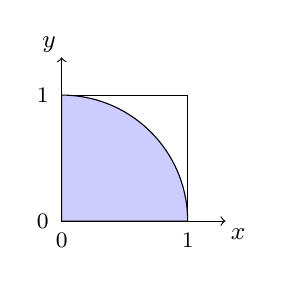
\begin{tikzpicture}[scale = 1.6]
\draw[thin] (0,0) -- (0,1) -- (1,1) -- (1,0) -- cycle; 
\filldraw[fill=blue!20!white, draw=black]
  (0,0) -- (1,0) arc (0:90:1) -- cycle;
\draw (0,\dd) node {\footnotesize $0$}; \draw (1,\dd) node {\footnotesize $1$};
\draw (\dd,0) node {\footnotesize $0$}; \draw (\dd,1) node {\footnotesize $1$};
\draw[->] (0,0) -- (1.3,0); \draw (1.4,-0.1) node {\small $x$};
\draw[->] (0,0) -- (0,1.3); \draw (-0.1,1.4) node {\small $y$};
\end{tikzpicture}
\end{myminipage}

\smallskip

The program below uses the bag-of-tasks pattern.  Each task is to generate
\SCALA{taskSize} pairs $(x,y)$ and to count how many satisfy $x^2+y^2 < 1.0$.
The controller sends a signal to a worker on |toWorkers| to tell it to perform
another task.  After |numTasks| such signals, it closes |toWorkers|, and each
worker sends its own count to the controller on |toController|.  The
controller than calculates the estimate of~$\pi$.   
%
\begin{scala}
object Pi{
  val taskSize = 400000 // Size of a single task.
  val numTasks = 200    // Number of tasks.
  val numWorkers = 8    // Number of workers.

  val toWorkers = new BuffChan[Unit](numWorkers)
  val toController = new BuffChan[Int](numWorkers)

  def worker = thread("worker"){
    val random = new scala.util.Random; var count = 0
    repeat{
      toWorkers?()
      for(i <- 0 until taskSize){
	val x = random.nextDouble(); val y = random.nextDouble()
	if(x*x + y*y < 1.0) count += 1
      }
    } // End of £repeat£ loop.
    toController!count
  }

  def controller = thread("controller"){
    for(i <- 0 until numTasks) toWorkers!()
    toWorkers.endOfStream()
    var count = 0
    for(i <- 0 until numWorkers) count += (toController?())
    println(4.0*count.toDouble/(taskSize*numTasks))
  }

  def system = controller || (|| ( for(i <- 0 until numWorkers) yield worker))

  def main(args: Array[String]) = run(system)
}
\end{scala}

We could have split the controller between two threads, and encapsulated each
into a separate object.

The above code gives each worker its own random number generator (RNG).  An
alternative is for the workers to share a single RNG.  However, my informal
experiments showed that the latter approach is about 20 times slower!  I think
the reason for this is that, when sharing, the state of the RNG has to be
copied to the cache of the relevant worker for each random number, and this is
slow.  When each worker has its own RNG, the state of that RNG will reside in
the worker's cache, and does not need to be reread from main memory.  

In fact, we should worry about whether sharing an RNG might constitute a race,
since the state of the RNG is updated for each random number.  However, it
turns out that the implementation does this in a thread-safe way.
\end{answerS}



%% If we let $n$ be the number of samples, then the number of samples that
%% satisfy the property $x^2+y^2<1$ has binomial distribution $Binom(n,\pi/4)$,
%% which has variance $n.\pi/4.(1-\pi/4)$, standard deviation
%% $\sqrt(n.\pi/4.(1-\pi/4))$, and so a standard deviation on the final result of
%% $4.\sqrt(\pi/4.(1-\pi/4)) / \sqrt n \approx 1.64 / \sqrt n$.  For $n = 10^6$, as
%% above, this is about $0.00164$.  This is consistent with the experimental
%% observation that the program is normally accurate to about two decimal places.
